\chapter{Dynamic Instrumentation Using Code Analysis And Transformation For Detailed GPU Communication Analysis}
This chapter describes in detail how the instrumentation works and will do so in the same order of steps as how an application is processed to generate traces.
First, the original application is instrumented on AST and LLVM IR level for tracing, then the data is generated on the GPU during the execution and transported to the host where it is stored in the trace file.
Global memory (see \ref{...}) is the only address space that is capable of enabling communication between
CTAs in an application and therefore is the only address space which memory operations will be instrumented
with tracing.

As libraries present external code not in source or LLVM IR, code using libraries can not be reliably instrumented.
%
%Figure \ref{compilestack} shows the necessary steps to add tracing to an application. The first step performs source-to-source compilation that augments the following kinds of statements in the original source with instructions required
%for tracing.
%
%These augmentations have to be performed for each file that contains either of the above statements individually because the process generated new files
%rather than overwriting the original source files. More details on the matter in section \ref{sec:impl:clang}
%

\begin{table}
\begin{tabular}{|c|c|c|c|c|c|c|}
	\hline 
	Name & Scope & Access & Bandwidth & Latency & Capacity & Location \\ 
	\hline 
	Shared Memory & CTA & RAM & high & low & low (48k) & Streaming Multiprocessor \\ 
	\hline 
	Global Memory & GPU & RAM & high & high & medium & device \\ 
	\hline 
	Texture/Constant & GPU & ROM & high & high & medium & device \\ 
	\hline 
	Host-Mapped Memory & GPU+CPU & RAM & low & high & high & host \\ 
	\hline 
\end{tabular} 
\caption{GPU Memory Types, move to Background chapter}
\label{GPUMemTable}
\end{table}



%The next step is the introduction to 
%
%Then explain how the tracing is introduced into the application
%\begin{enumerate}
%	\item Generate object files from augmented source files and insert tracing with LLVM Plugin:
%	\item Linking
%\end{enumerate}


\section{Source to Source Compilation in CLang}\label{sec:impl:clang}
%The first instrumentation step extends the original source code with the information for the buffers used during the trace, specifically the items listed below.
%\begin{itemize}
%	\item Kernel Declarations
%	\item Kernel Definitions
%	\item Kernel calls
%	\item \verb|__device__| function declaration
%	\item \verb|__device__| function definitions
%	\item \verb|__device__| Function calls inside a Kernel
%\end{itemize}
%
%
%\begin{itemize}
%	\item User has to know which files need augmentation
%	\item Augmentation of one file at a time, since out-of-place code transformation is performed
%	\item Working in Clang AST
%	\item Find all places in the code that need Augmentation:
%	\begin{enumerate}
%		\item Kernel Definition: Add set of arguments used for tracing
%		\item Kernel Calls: Add arguments used for tracing
%		\item Include File offering the tracing utils
%	\end{enumerate}
%\end{itemize}
\section{Code Transformation in LLVM}
Instrumenting the application to generate trace data for global memory operations on the GPU happens inside a LLVM IR optimisation pass. The original source is analysed and instrumented at the locations of loads, stores and atomic operations targeting global memory, so that during the execution data is generated.

Global memory is the only address space of CUDA in which side effects that are visible across kernel completion boundaries are possible. These side effects can carry information from a kernel to another and so memory operations using this address space need instrumentation. Clang performs lowering of all memory access operations during the generation of LLVM IR and in the process eliminates the address space information at location of the memory operation. An example for the lowering is displayed in listing \ref{lowering}, showing that the information is 'casted' away by the IR. The \verb|getelementptr| instruction is used
for address calculation, for example to access a specific element in an array. However, before this is done
the address space of the original pointer is lowered to the generic address space by \verb|addrspacecast|. The pointer used in the \verb|store| instruction in line two does not contain information about it's address space.
 
PTX does not necessarily need address space information for a memory operation since it can be resolved dynamically during runtime. While PTX has distinct load (\verb|ld|) and store (\verb|st|) instruction for
each address space, a generic version is also available. This generic instruction maps to global memory, if
it does not fit into a window for the other address spaces \cite{ptx isa}. This lookup however comes at the cost of a minor performance decrease \cite{infer-pass}. So, while beneficial it is not necessary to
have the address space information to build a correct application. For the tracing process however, we need to have this information to prevent the generation of trace data for parts of the address space that are not interesting for this work.

\begin{figure}
	\begin{lstlisting}[style=C]
%arrayinx1 = getelementptr inbounds (float, float* addrspacecast (float addrspace(3)* @_ZZ5saxpyfPfS_iPlS0_E2_x to float*), i64 0, i64 2)
store float 1.000000e+00, float* %arrayinx1
	\end{lstlisting}
	\caption{Example for address space lowering in LLVM IR}
	\label{lowering}
\end{figure}

There is an experimental LLVM optimizer pass which tries to infer the address space by analysing the steps that have been introduced by the lowering. However, it works on a function scope which is not sufficient for our purposes. Address space information  might not be existing in the function argument because of lowering of the argument previous to the function call. And due to the pass' function scope, information on the calling context is not available. Because the pass can fall back to the generic address space,
it is not critical if the address space can not be determined reliably. This is not sufficient for the needs of this work.
Therefore an  analysis is performed, that generates definitive information, whether a memory access targets
global memory or not. If generating this information is not possible, the pass fails. The reason for an unsuccessful execution is  explained in section \ref{pa}, after more details of the actual analysis have been explained.

LLVM widest analysis scope is 'Module', which roughly corresponds to one translation unit in C. Interactions of the original source that reach beyond this Module scope can not be analysed, and therefore not instrumented.

\subsection{Address Space Analysis}\label{pa}
The basic principle of this analysis rests on the limited number of sources in 
a kernel, where a global address space pointer can be obtained from.
\begin{itemize}
	\item direkt kernel parameters
	\item indirekt kernel parameters (struct etc.)
	\item global variables
	\item pointer type load from global memory
\end{itemize}
Collecting base pointers form all these sources provides starting points for a sparse analysis of the program,
because only memory operations that are part of def-use chains rooting in these base pointers, can be a candidate for instrumentation.

%	\begin{defi}
%	$	MOp = \{\textrm{LoadInst, StoreInst, atomicInst}\} $
%	\end{defi}
%	\begin{defi}
%	$   POp = \{ \textrm{LoadInst of Type Ptr, GetElementPtr, CastInst, Arg of CallInst} \} $
%	\end{defi}
%	\begin{defi}
%	$	NMOp = \{inst : inst \notin POp, inst \notin MOp\}$
%	\end{defi}


%	\centering
%	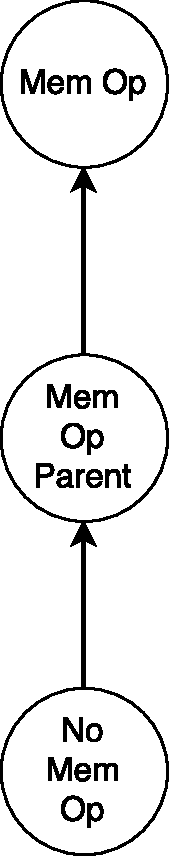
\includegraphics[height=0.3\textwidth]{lattice}
%	\caption{Property space lattice}
%	\label{ptr-analysis}

The used algorithm performs a 'must'-analysis on the sparse problem space that is represented by the def-use chains created by the SSA form of LLVM IR. Because the the algorithm follows the order of instructions through the program, it can be described as 'flow sensitive'. Function calls are only
analysed if they happen in a 'global-memory context' which in our case means that one of arguments used in the call is a pointer to global memory. This classifies our algorithm as 'context sensitive'.
The property space of the analysis describes sets of instructions in the context of global memory operations that are defined
as following:
\begin{defi}\label{mop}
	$	MOp = \{\textrm{LoadInst, StoreInst, CallInst}\} $
\end{defi}
$MOp$ contains all types of instruction, that are interesting for tracing. During the analysis they are marked for later instrumentation. LLVM maps CUDA's atomic operations to functions, which is why $\textrm{CallInst}$ is part of this set. Of course they are only considered a memory access, if the callee is an atomic function.
\begin{defi}\label{mopp}
	$   POpP = \{\textrm{CallInst, GEPInst, CallInst, PHINode, SelectInst}\} $
\end{defi}
$POp$ contains operations that define new SSA variables which can be used in operations interesting for tracing. $CastInst$ because of the lowering  and $GEPInst$ since it is the generic way in LLVM
to perform address arithmetic. Their users need to be visited later. 
$PHINode$ and $SelectInst$ are special cases. Only instructions that resolve pointers and all arguments can be related to a global memory base pointers are a part of this set. The reason for
this is explained in section \ref{patho}.
This set also includes function calls. However, in the case of a function not the return value definition, but the argument passed into the function marked for later analysis. More on the return values of functions in section \ref{patho}.
\begin{defi}\label{nmop}
	$	NMOp = \{inst : inst \notin POp, inst \notin MOp\}$
\end{defi}
$NOp$ contains all instructions that are of no interest for the analysis and are ignored.

To obtain a list of all instruction which require instrumentation, each of the orginal base pointers is handled by Algorithm \ref{anal-algo} to create list of all descendant memory operations of the original by applying the transfer function $f(x)$ to every instruction processed. $f(x)$ classifies each instruction, assigning it to one of the three sets $MOp$, $POp$ or $NOp$. After this is done for each function a list with the instructions has been generated, which is then
used for instrumentation. This algorithm only proves if a memory operation uses a pointer originating from a original base pointer, and therefore uses the same address space, which can be achieved without the need to analyse cycles in the CFG. As a consequence the algorithm always terminates once each instruction is visited. 
By keeping track of each function that was already visited, recursion is not an issue during the analysis.


\begin{algorithm}[t]
\KwData{orignal pointer}
\KwResult{List of global memory operations based on original pointer }
add original pointer to workstack\;
\While{workstack not empty}{
	get element form workstack\;
	\ForAll{users of element} {
	\tcc{apply tranfer function $f(x)$ to user:}
	\uIf{$type(user) \in MOp$}{
		add user to list for tracing\;
	}\uElseIf{$type(user) \in POp$}{
		add new parent to workstack\;
	}\uElseIf{$type(user) \in NOp$}{
		continue with next user\;
	}

}
}
\caption{How to find global memory operations based on a input pointer}
\label{anal-algo}
\end{algorithm}
\paragraph{$\phi$-Node Limitations}\label{patho}
Static analysis has some limitations that can cause an unsuccessful address space analysis. This particular issue is caused by the SSA's need to define a new version for a variable each time said variable changes. This results in the need of $\phi$-functions and \verb|select| statements, which is a LLVM IR instruction to handle small \verb|if-else| branches without the need for multiple basic blocks
and a $\phi$-node. Figure \ref{phinodes} shows a minimal code example that can lead to a situation which is not analysable by our static analysis, because it requires resolving pointers to different address spaces at runtime. The code sample on the left creates a situation where a $\phi$-node is required to resolve the edges of the incoming basic blocks. Each of these basic blocks defines a surrogate pointer for \verb|d|. For this example we will call them \verb|ds1| and \verb|ds2|. Based on \verb|ds1| and \verb|ds2| the $\phi$-node defines a pointer \verb|df| that is used for the following operations performed on \verb|d|. Therefore the $\phi$-node resolves which address space \verb|df| points to. 

This is illustrated by graphs on the right hand side of the figure. Every block preceding the $\phi$-node carries an address space, represented by a colour.
The left graph has to resolve different address spaces and therefore the address space for \verb|df| is ambiguous. This leads to an unsuccessful analysis. The right graph shows a special case the implemented pass can resolve by proving that \verb|ds1| and \verb|ds2| both point to the same address space, which concludes that \verb|df|'s address space is definite. The proof is implemented as a table counts how often the analysis pass visits every phi-node. After the analysis is finished the value in the table is compared to the $\phi$-nodes incoming edges. If the counted value and number of edges match the pass proved the special case, otherwise we have ambiguity in the address space of \verb|df|, which leads to aborting the instrumentation pass.

\begin{figure}[t]
		\begin{minipage}{0.35\textwidth}

		\begin{lstlisting}[style=c]
__global__ float *gx;
__shared__ float *sx;
float *d;
if (a > b)
	d = gx;
else 
	d = sx;
		\end{lstlisting}
			\end{minipage}\hfill
	\begin{minipage}{0.6\textwidth}
		\centering
		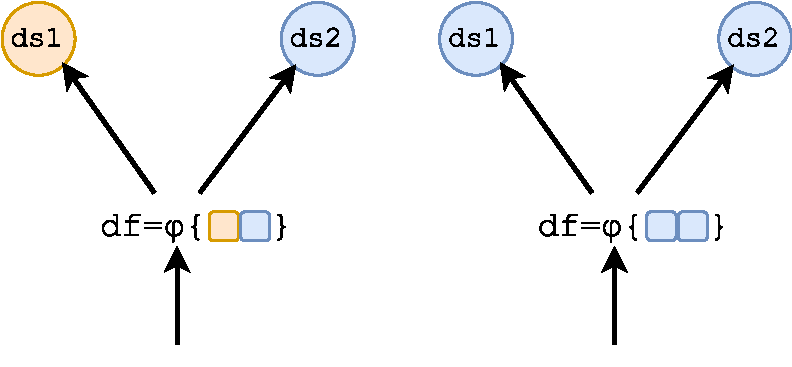
\includegraphics[width=\textwidth]{phinode2}
	\end{minipage}\hfill
	\caption{Example for static analysis limitations. Different colors represent different address spaces. The left graph represents the generic problem case and right graph a special case that is resolvable by the analysis.}
	\label{phinodes}
\end{figure}

\paragraph{Ambiguous Function Address Space}\label{func-vers}
Another issue is possible ambiguity in the address space of pointers that are passed to functions. To illustrate this issue, figure \ref{func-vers} provides on the left hand side a code sample of a coalescing copy function. CUDA allows calling this device function with pointers to every address space and every combination of address spaces. The kernel on the right hand side then uses the function twice, once to copy data from the global memory into shared memory and a second time to move the data back to the global memory.

Now the instrumentation pass analyses the kernel and finds the first function call and sees that a function is called and the first
parameter is a global memory pointer. It enters the function and marks the \verb|load| instruction for tracing. The pass continues and later finds a call to the same function, enters the function again and this time marks the \verb|store| for tracing, because the pointer
led the pass to it. Now both memory operations are marked as global memory operations and generate trace data, although they are not always used with a global address space pointer. This issue is the reason, our needs to be context sensitive.

\begin{figure}[t]
	\begin{minipage}{0.45\textwidth}
		
		\begin{lstlisting}[style=c]
void copy(float* src, float* dst) {
	dst[tix] = src[tix];
}
		\end{lstlisting}
	\end{minipage}\hfill
	\begin{minipage}{0.45\textwidth}
			\begin{lstlisting}[style=c]
__global__ void k (float* gx) {
	__shared__ float* sx;
	copy(gx, sx);
	// kernel does stuff
	copy(sx, gx);
	return;
}
	\end{lstlisting}
	\end{minipage}\hfill
	\caption{Example for ambiguous function address spaces}
	\label{func-vers}
\end{figure}
\subsection{Instrumentation}\label{instru}
%Once all instruction of interest have been found, the actual transformation takes place.
%It is straight forward process and always consists of the same steps. 
%
%Before the tracing is added, for every function that contains an instruction that will be traced the following things
%are performed
%\begin{enumerate}
%	\item Fetch arguments from argument list, that has been added during the source to source compilation (see section \ref{sec:impl:clang})
%	\item Fetch SMID
%	\item Calculate base address of trace buffer from SMID and information fetched from the args.
%\end{enumerate}
                                                                

\section{Tracing Process}
	Many applications have non-deterministic executions, for example no predetermined number of kernel calls because of varying input data. Examples are graph algorithms depending on the underlying graph's structure or numerical solvers, which iterate until a
	convergence condition is reached by the residual. Because of this, a static buffer that is filled up once and is cleared at the end of the application does no suffice for reliable and dynamic tracing.
	
	Therefore a producer-consumer queue for the generated trace data between GPU and host is used that ensures the application never runs out of buffer space for the tracing data. The GPU generates the data and the host evacuates full buffers, storing the data.
	The buffer containing the generated data is host-mapped memory, which is separated into several bins. The bins are used to reduce
	pressure on the memory system that is generated by the atomic index accesses of the producer-consumer setup. The number of bins 
	is always a $2^n$ and a scheduled CTA uses the  $n$ least significant bits of the SM's ID it is scheduled on, to select a bin. Therefore the number of bins should be selected as the closest power of two, to the number of SMs.

	Writing the data to the disk after they have been cleared from the buffer by the consumer, showed to be a performance critical aspect during the trace. Per default, Linux directs \verb|writes()| to a page cache. Smaller, periodic writes (64Kbyte to 1Mybte) to the disk empirically showed to be more efficient. The author assumes this is caused by overlapping between cache management and queue management.
	
	\subsection{On-Device Producer}
\begin{figure}[t]
	\centering
	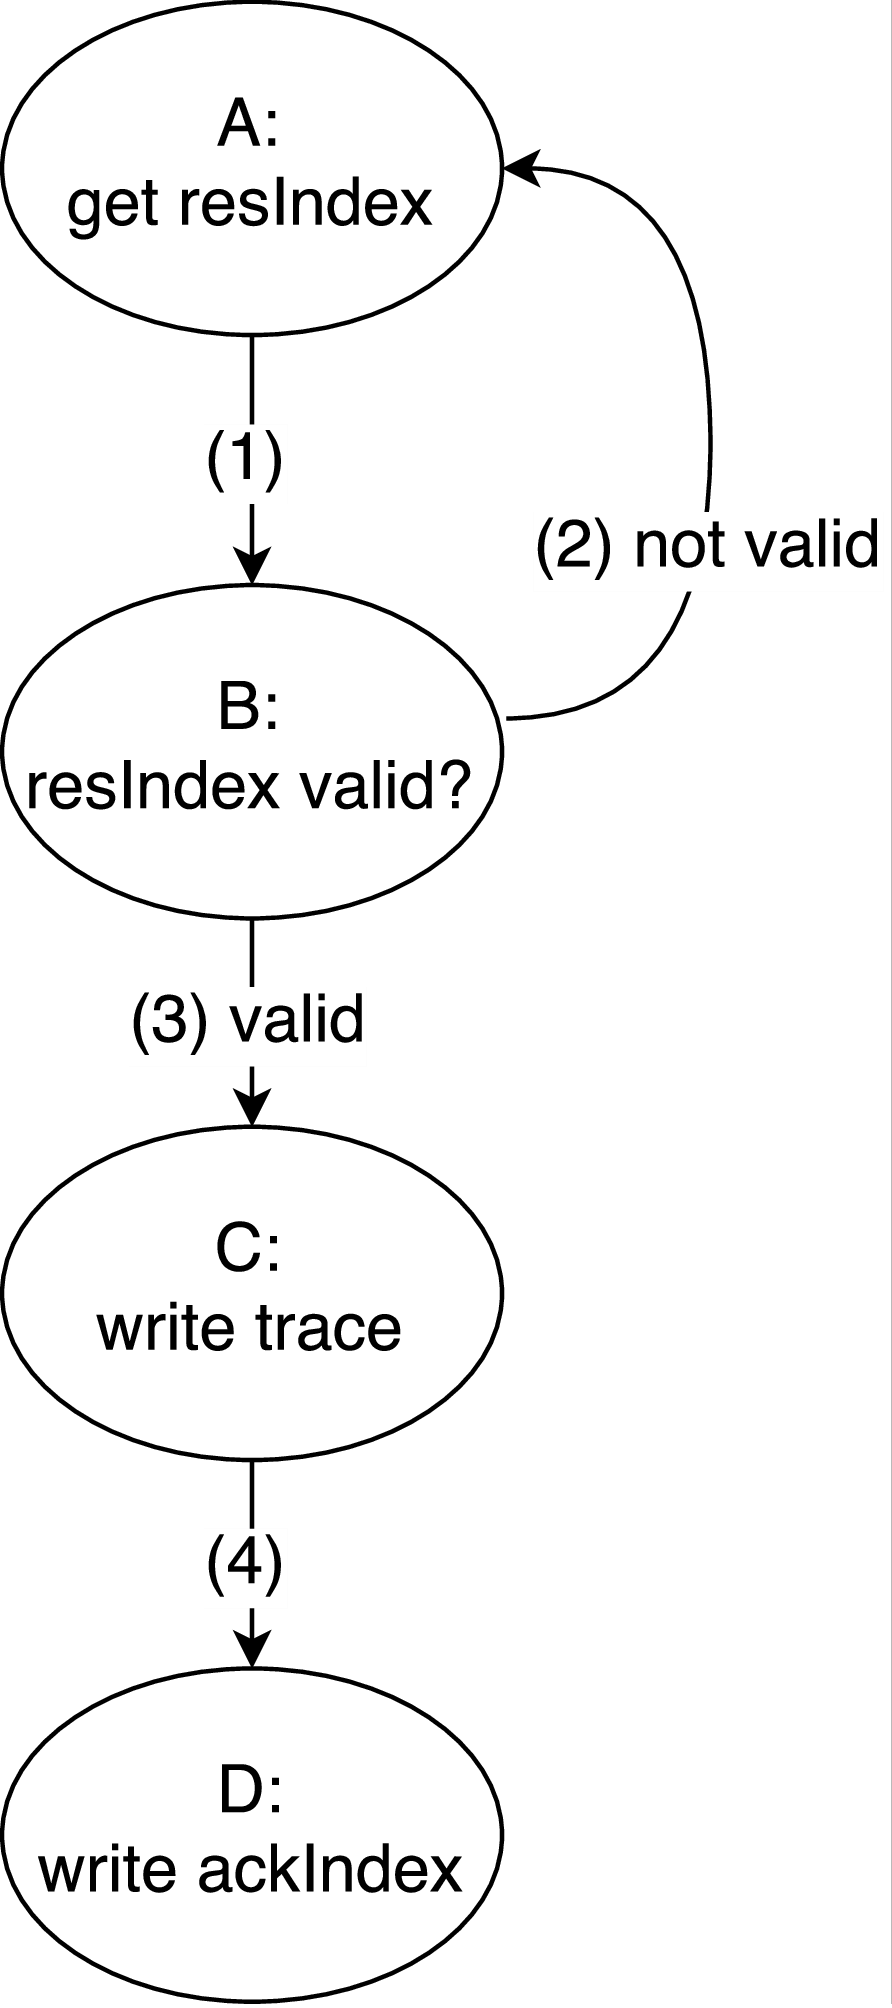
\includegraphics[width=0.3\textwidth]{warp-scope-cfg}
	\caption{Producer CFG}
\label{wscfg}
\end{figure}	
	This section focusses on the producer that is running on the device, making sure that data is only written if there space left
	in a buffer. The producer-consumer setup uses a head and a tail index to handle reservation of buffer space and write acknowledgements to signal that the write has completed. Code sample \ref{prod-cons} shows the pseudo-algorithm that is performed by the producer. First the required buffer space is reserved for writing by incrementing the reservation index
	by the number of required slots (line 1). Then the data generated by the trace is
	written to the buffer (line 2) and the write acknowledgement is incremented by the same number of buffer slots (line 3).
\begin{figure}
	\begin{lstlisting}[style=C]
while((ackIndex > maxIndex) or (id = atomicAdd(resIndex, increment) > maxIndex));
buffer[id] = traceData;
atomicAdd(ackIndex, increment);
\end{lstlisting}
	\caption{Device Producer, naive approach}
	\label{prod-cons}
\end{figure}

	
	This is implemented on a warp scope, which means either the whole warp continues or waits, to prevents deadlocks during indices fetching.
	A deadlock can occur because of how GPUs manage branch divergence inside a warp. If the instruction stream of a warp branches, all member threads of this warp execute both branches, and the group of members that should not be executing this part of the code is masked out. After all branches completed execution, the combined execution of both groups continues.
	
	A deadlock can occur, if each thread fetches it's \verb|resIndex| individually and there is not enough available buffer space for all threads inside the warp. Referring to figure \ref{wscfg} now, all threads will execute edge (1) leading from (A) to (B) by fetching \verb|resIndex|. If all threads get a valid index (B), the warp will not branch and the trace can complete successfully.
	If the check in (B) fails for one or more threads in the warp, a branch is created. The branch without valid IDs will 
	use edge (2), returning to node (A) and retry fetching a valid \verb|resIndex|. The branch with valid \verb|resIndex|
	has to wait with progressing on edge (3) until the group without valid \verb|resIndex| is also ready to continue on edge (3).
	But because the warp can not progress over edge (3) to and C and from there over (4) to D, until all threads have a valid \verb|resIndex|, the threads in the warp that already have a valid \verb|resIndex| can not reach node D write \verb|ackIndex|, which would lead to a evacuation of the buffer on by the host and a reset of the \verb|achIndex| and \verb|resIndex|. As a result of this, a deadlock occurs because one group of threads waits for a resource that can not be released by the other group
	of threads due to the warp execution model.
	
	This can be resolved by handling reservation and write acknowledgement on a warp level. One thread makes the reservation and write the acknowledgement for all threads inside the warp. Now either the whole warp can finish the trace or the whole warp stalls. This way we can use the warp execution model for our purposes, because one thread that waits for the IDs can stall the whole warp with an if branch and no other means of synchronization. This is implemented by using CUDA warp intrinsics, which offer efficient communication inside of warps.
\begin{figure}[t]
	\begin{lstlisting}[style=C]
active   = __ballot(1); // get bitmap of active threads 
nActive  = __popc(active); // get count of active threads
lowest   = __ffs(active)-1; // check which thread has to perform sync
rlane_id = __rlaneid(active, lane_id); // each thread gets its relative Lane id, based on number of active threads
	
if (lane_id == lowest)
	while( ackIndex >= maxIndex-maxWarpWrite 
		|| (id = atomicAdd(resIndex, nActive)) >= maxIndex-maxWarpWrite
	);
// Warp stalls here until all branch is completed

idx = __shfl(id, lowest) + rlane_id; // distribute id
buffer[id] = traceData;
if (lane_id == lowest )
	atomicAdd(ackIndex, n_active);
	\end{lstlisting}
	\caption{Device Producer, warp scope}
	\label{prod-cons-warp}	
\end{figure}
	Little extra code is needed shift everything to a warp-scope management, as seen in Figure \ref{prod-cons-warp}. Because it is possible that a trace occurs on a point during the execution, where the warp is already branched we have to make sure
	that the indexes are managed correctly and only the currently active threads participate in the trace. The warp intrinsics \verb|__ballot|, \verb|__popc| and \verb|__ffs| are used to determine how many threads are active, and which one has to perform the atomic operations to handle
	the producer synchronization. Then \verb|__rlaneid()|, which is user code, calculates the relative lane id for each warp. 
	
	While the lowest thread fetches the id for the buffer using \verb|atomicAdd|, the whole warp stalls at the end of the if clause because of the warp execution model. Once a valid id is fetched, it is distributed among all threads using the \verb|__shfl| intrinsic. 	Then the trace is written and the lowest thread increments the write acknowledgement by the number it increased the reservation.
	
	Notice that in this case, the conditions for fetching the id now takes into account that data is written in blocks and has to check if there is still space left for one complete block. 
	
	Assuming a warp is fully populated warp at the moment a trace happens and thus always reserve enough buffer space for a whole warp can create gaps in the trace data. To prevent old data from lingering, the buffer would need to be wiped after every evacuation of the
	generated trace data. Additionally, these gaps would require additional handling in the analysis of the data.
	Therefore, this more complex approach of handling the consumer was chosen, which only reserved as much space as required.

	
	\subsection{Host Consumer}
	The consuming thread on the host side is much simpler. A single thread is iterating over all bins in the buffer, checking if the
	\verb|ackIndex| is at the threshold for evacuation. This threshold is reached if there is not enough space for a complete warp to
	write a trace.
	The buffer is evacuated by writing the data into a file handle and \verb|resIndex| and \verb|ackIndex| reset to the beginning of the buffer.
%	
%	...
%
%\begin{itemize}
%	\item General Tracing Setup
%	\item Producing Data on the Device: Handling Indices on a Warp Scope
%	\item Consuming data on the host side
%	\item Handling Streams
%\end{itemize}
%

